\documentclass[lang=cn, thmcnt=section, chinesefont=founder, color=cyan, citestyle=gb7714-2015, bibstyle=gb7714-2015]{elegantbook}

\usepackage{unicode-math}
\setmathfont{STIXTwoMath-Regular.otf}

\usepackage{minted}
\usepackage[color=black]{siunitx}
\usepackage[ISO]{diffcoeff}
\usepackage{tikz}
\usepackage{tkz-euclide}
\usepackage{tkz-graph}
\usepackage{dashrule}
\usepackage{float}

\PassOptionsToPackage{dvipsnames,svgnames,x11names}{xcolor}

\definecolor{shadow}{RGB}{210,241,241}

\titleformat{\chapter}[display]{\vspace*{\fill}\bfseries}{
  \hspace*{\fill}\zihao{1}\enspace\bfseries{\color{structurecolor} \IfAppendix{\appendixname\;\thechapter\;}{\xchaptertitle}}}{0pt}{
  \hspace*{\fill}\zihao{-0}\bfseries\color{black}}[\vspace{-1em}\color{structurecolor}\rule{\textwidth}{2pt}\vspace*{\fill}\newpage]
\titleformat{\section}[hang]{\bfseries}{
  \filcenter\LARGE\bfseries{\color{structurecolor}\thesection}\enspace}{1pt}{%
  \color{structurecolor}\LARGE\bfseries\filcenter}
\titleformat{\subsection}[hang]{\bfseries}{
  \Large\bfseries\color{structurecolor}\thesubsection\enspace}{1pt}{%
  \color{structurecolor}\large\bfseries\filright}
\titleformat{\subsubsection}[hang]{\bfseries}{
  \large\bfseries\color{structurecolor}\thesubsubsection\enspace}{1pt}{%
  \color{structurecolor}\large\bfseries\filright}

\tcbuselibrary{minted}
\newcommand{\spare}{\vspace{-1em}\begin{center}\color{structurecolor}\hdashrule[0.5ex]{\textwidth}{1pt}{1pt}\end{center}\vspace{-1em}}
\usetikzlibrary{shapes,backgrounds}
\ExecuteBibliographyOptions{sorting=gb7714-2015}
\setlength{\parskip}{1ex}
\newtcolorbox{collections}{
      boxrule=0.5pt,
      enhanced,
      breakable,
      top=8pt,
      before skip=8pt,
      colframe=structurecolor,
      colback=structurecolor!5,
      colbacktitle=structurecolor
}
\newtcblisting{code*}[1]{
    listing engine=minted,
    boxrule=0.1mm,
    colback=third!5,
    colframe=third,
    listing only,
    left=5mm,
    enhanced,
    breakable,
    overlay={\begin{tcbclipinterior}\fill[third] (frame.south west)
    rectangle ([xshift=5mm]frame.north west);\end{tcbclipinterior}},
    minted language=#1,
    minted style=vs,
    minted options={breaklines, mathescape, autogobble, linenos, numbersep=2mm}
}
\newtcblisting[auto counter]{code}[2]{
    listing engine=minted,
    boxrule=0.1mm,
    colback=third!5,
    colframe=third,
    listing only,
    left=5mm,
    enhanced,
    breakable,
    title=Program \Alph{\tcbcounter}: #2,
    overlay={\begin{tcbclipinterior}\fill[third] (frame.south west)
    rectangle ([xshift=5mm]frame.north west);\end{tcbclipinterior}},
    minted language=#1,
    minted style=vs,
    minted options={breaklines, mathescape, autogobble, linenos, numbersep=2mm}
}
\renewcommand{\theFancyVerbLine}{\textcolor{white}{\footnotesize{\arabic{FancyVerbLine}}}}

\renewcommand{\bar}[1]{\overline{#1}}
\arrayrulecolor{second}

\usetikzlibrary{graphs}

\title{新世代计算机科学计划·基础篇}
\author{JouderMin}
\institute{「新世代计算机科学计划」制作委员会}
\date{\zhtoday}
\cover{img/cover.png}
\logo{img/方形logo.png}

\begin{document}
\maketitle
\frontmatter

\tableofcontents

\mainmatter

\chapter{离散数学}
\input{SectionPage/1.1.tex}
\input{SectionPage/1.2.tex}
\input{SectionPage/1.3.tex}
\section{图的表示}
\begin{introduction}
    \item 邻接表
    \item 邻接矩阵
    \item 关联矩阵
\end{introduction}
\subsection{邻接表}
邻接表可以用来表示不存在多重边的图。
\begin{collections}
    \begin{example}
        用邻接表表示以下无向图。
        \vspace{-2em}
        \begin{center}
            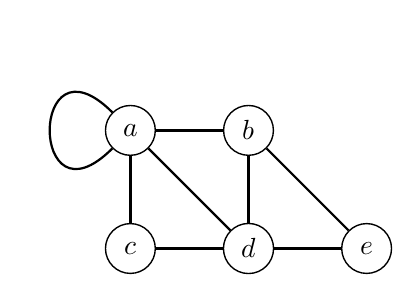
\begin{tikzpicture}
                \GraphInit[vstyle=normal]
                \SetGraphUnit{1.5}\SetVertexMath
                \Vertex{a}
                \EA(a){b}
                \SO(a){c}
                \EA(c){d}
                \EA(d){e}
                \Edge[style={-}](a)(b)
                \Edge[style={-}](a)(c)
                \Edge[style={-}](a)(d)
                \Edge[style={-}](b)(d)
                \Edge[style={-}](b)(e)
                \Edge[style={-}](c)(d)
                \Edge[style={-}](d)(e)
                \Loop[style={-},dist=1.5cm](a)
            \end{tikzpicture}
        \end{center}
    \end{example}
    \begin{solution}
        \begin{center}
            \begin{tabular}{c|c}
                \toprule
                \makebox[2cm][c]{顶点} & \makebox[2cm][c]{邻居} \\
                \midrule
                $a$ & $a, b, c, d$ \\
                $b$ & $a, d, e$ \\
                $c$ & $a, d$ \\
                $d$ & $a, b, c, e$ \\
                $e$ & $b, d$\\
                \bottomrule
            \end{tabular}
        \end{center}
    \end{solution}

    \spare

    \begin{example}
        用邻接表表示以下有向图。
        \vspace{-2em}
        \begin{center}
            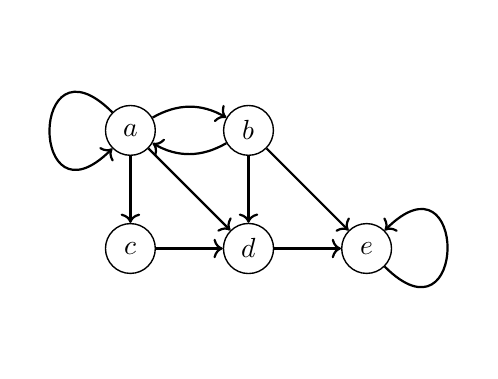
\begin{tikzpicture}
                \GraphInit[vstyle=normal]
                \SetGraphUnit{1.5}\SetVertexMath
                \Vertex{a}
                \EA(a){b}
                \SO(a){c}
                \EA(c){d}
                \EA(d){e}
                \Edge[style={->, bend left}](a)(b)
                \Edge[style={->, bend left}](b)(a)
                \Edge[style={->}](a)(c)
                \Edge[style={->}](a)(d)
                \Edge[style={->}](b)(d)
                \Edge[style={->}](b)(e)
                \Edge[style={->}](c)(d)
                \Edge[style={->}](d)(e)
                \Loop[style={->},dist=1.5cm](a)
                \Loop[style={->},dist=1.5cm, dir=EA](e)
            \end{tikzpicture}
            \vspace{-2em}
        \end{center}
    \end{example}
    \begin{solution}
        \begin{center}
            \begin{tabular}{c|c}
                \toprule
                \makebox[2cm][c]{起点} & \makebox[2cm][c]{终点} \\
                \midrule
                $a$ & $a, b, c, d$ \\
                $b$ & $a, d, e$ \\
                $c$ & $d$ \\
                $d$ & $e$ \\
                $e$ & $e$ \\
                \bottomrule
            \end{tabular}
        \end{center}
    \end{solution}
\end{collections}

\subsection{邻接矩阵}
当图中边的数量较多时,可以使用邻接矩阵来表示图。

无向图 $G=(V, E)$ 的邻接矩阵是一个大小为 $|V| \times |V|$ 的矩阵,矩阵中的元素 $a_{ij}$ 表示顶点 $v_i$ 与 $v_j$ 之间边的数量。无向图的邻接矩阵是关于其主对角线对称的。

有向图 $G=(V, E)$ 的邻接矩阵也是一个大小为 $|V| \times |V|$ 的矩阵,不过矩阵中的元素 $a_{ij}$ 表示以顶点 $v_i$ 为起点,$v_j$ 为终点的边的数量。有向图的邻接矩阵不一定是对称的。
\begin{collections}
    \begin{example}
        用邻接矩阵表示以下无向图。
        \vspace{-2em}
        \begin{center}
            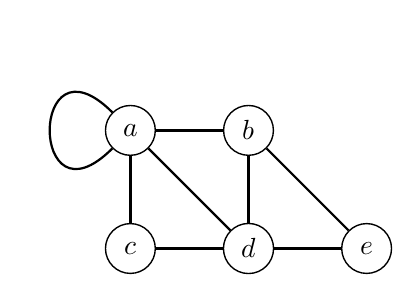
\begin{tikzpicture}
                \GraphInit[vstyle=normal]
                \SetGraphUnit{1.5}\SetVertexMath
                \Vertex{a}
                \EA(a){b}
                \SO(a){c}
                \EA(c){d}
                \EA(d){e}
                \Edge[style={-}](a)(b)
                \Edge[style={-}](a)(c)
                \Edge[style={-}](a)(d)
                \Edge[style={-}](b)(d)
                \Edge[style={-}](b)(e)
                \Edge[style={-}](c)(d)
                \Edge[style={-}](d)(e)
                \Loop[style={-},dist=1.5cm](a)
            \end{tikzpicture}
        \end{center}
    \end{example}
    \begin{solution}
        $$
        \begin{bmatrix}
            1 & 1 & 1 & 1 & 0 \\
            1 & 0 & 0 & 1 & 1 \\
            1 & 0 & 0 & 1 & 0 \\
            1 & 1 & 1 & 0 & 1 \\
            0 & 1 & 0 & 1 & 0 \\
        \end{bmatrix}
        $$
    \end{solution}

    \spare

    \begin{example}
        用邻接矩阵表示以下有向图。
        \vspace{-2em}
        \begin{center}
            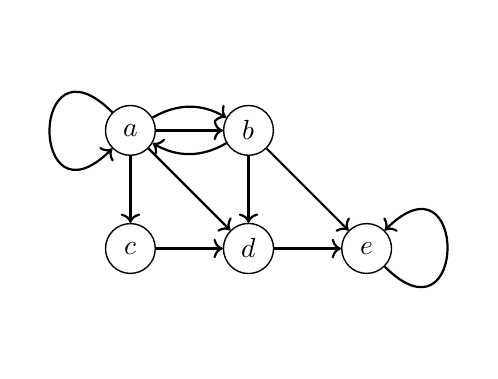
\begin{tikzpicture}
                \GraphInit[vstyle=normal]
                \SetGraphUnit{1.5}\SetVertexMath
                \Vertex{a}
                \EA(a){b}
                \SO(a){c}
                \EA(c){d}
                \EA(d){e}
                \Edge[style={->}](a)(b)
                \Edge[style={->, bend left}](a)(b)
                \Edge[style={->, bend left}](b)(a)
                \Edge[style={->}](a)(c)
                \Edge[style={->}](a)(d)
                \Edge[style={->}](b)(d)
                \Edge[style={->}](b)(e)
                \Edge[style={->}](c)(d)
                \Edge[style={->}](d)(e)
                \Loop[style={->},dist=1.5cm](a)
                \Loop[style={->},dist=1.5cm, dir=EA](e)
            \end{tikzpicture}
            \vspace{-2em}
        \end{center}
    \end{example}
    \begin{solution}
        $$
        \begin{bmatrix}
            1 & 2 & 1 & 1 & 0 \\
            1 & 0 & 0 & 1 & 1 \\
            0 & 0 & 0 & 1 & 0 \\
            0 & 0 & 0 & 0 & 1 \\
            0 & 0 & 0 & 0 & 1 \\
        \end{bmatrix}
        $$
    \end{solution}
\end{collections}

可以看出,对于无向图的邻接矩阵,存在
\begin{equation*}
    \sum_{j=1}^{|V|}(a_{ij} + a_{ji})=\symrm{deg}(v_i)
\end{equation*}
对于有向图的邻接矩阵,存在
\begin{equation*}
    \begin{aligned}
        \sum_{j=1}^{|V|}a_{ij}=\symrm{deg}^+(v_i) \\
        \sum_{j=1}^{|V|}a_{ji}=\symrm{deg}^-(v_i) \\
    \end{aligned}
\end{equation*}

\subsection{关联矩阵}
关联矩阵于邻接矩阵不同,关联矩阵只能用于表示无向图。设无向图 $G=(V,E)$,其关联矩阵是一个大小为 $|V|\times|E|$ 的 $01$ 矩阵,矩阵中的元素 $a_{ij}$ 有以下特点。
\begin{equation*}
    a_{ij}=
    \begin{cases}
        1 & \text{$v_i$ 与 $e_j$ 相关联} \\
        0 & \text{$v_i$ 与 $e_j$ 无关} \\
    \end{cases}
\end{equation*}

\begin{collections}
    \begin{example}
        用关联矩阵表示以下无向图。
        \vspace{-2em}
        \begin{center}
            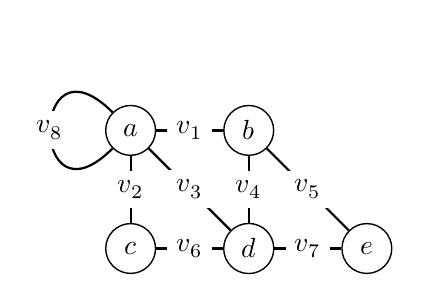
\begin{tikzpicture}
                \GraphInit[vstyle=normal]
                \SetGraphUnit{1.5}\SetVertexMath
                \Vertex{a}
                \EA(a){b}
                \SO(a){c}
                \EA(c){d}
                \EA(d){e}
                \Edge[style={-}, label={$v_1$}](a)(b)
                \Edge[style={-}, label={$v_2$}](a)(c)
                \Edge[style={-}, label={$v_3$}](a)(d)
                \Edge[style={-}, label={$v_4$}](b)(d)
                \Edge[style={-}, label={$v_5$}](b)(e)
                \Edge[style={-}, label={$v_6$}](c)(d)
                \Edge[style={-}, label={$v_7$}](d)(e)
                \Loop[style={-}, labelstyle={fill=white}, label={$v_8$}, dist=1.5cm](a)
            \end{tikzpicture}
        \end{center}
        \begin{solution}
            $$
            \begin{bmatrix}
                1 & 1 & 1 & 0 & 0 & 0 & 0 & 1 \\
                1 & 0 & 0 & 1 & 1 & 0 & 0 & 0 \\
                0 & 1 & 0 & 0 & 0 & 1 & 1 & 0 \\
                0 & 0 & 1 & 1 & 0 & 1 & 0 & 0 \\
                0 & 0 & 0 & 0 & 1 & 0 & 1 & 0 \\
            \end{bmatrix}
            $$
        \end{solution}
    \end{example}
\end{collections}

\newpage

\section{图的连通性}
\begin{introduction}
    \item 通路与回路
    \item 无向图的连通性
    \item 有向图的连通性
\end{introduction}

\subsection{通路与回路}

\begin{definition}[无向图的通路与回路]\label{def:无向图的通路与回路}
    设 $n$ 是正整数且 $G=(V,E)$ 是无向图,$u,v \in V$。在 $G$ 中从 $u$ 到 $v$ 的长度为 $n$ 的通路指 $G$ 中边的序列 $(e_1,e_2,\cdots,e_n)$,其中边 $e_1$ 与顶点 $u$ 相关联,边 $e_n$ 与顶点 $v$ 相关联,根据这个边的序列,可以列出与每条边相关联的顶点序列 $(u,\cdots,v)$,当 $G$ 是简单无向图时,可以使用该顶点顶点序列来表示这条通路。如果一条通路在相同的顶点上开始和结束且该通路长度大于 $0$,则称这条通路是一条回路。若通路或回路中不包含相同的边,则称他是简单的。
\end{definition}

由定义 \ref{def:无向图的通路与回路} 我们可以类比作出有向图中通路与回路的定义。

\begin{definition}[有向图的通路与回路]\label{def:有向图的通路与回路}
    设 $n$ 是正整数且 $G=(V,E)$ 是有向图,$x_1,x_2,x_{n-1},x_n \in V$。在 $G$ 中从 $x_1$ 到 $x_n$ 的长度为 $n$ 的通路指 $G$ 中边的序列 $(e_1,e_2,\cdots,e_n)$,其中边 $e_1 = (x_1,x_2)$,边 $e_n = (x_{n-1},x_n)$,根据这个边的序列,可以列出与每条边相关联的顶点序列 $(x_1,x_2,\cdots,x_n)$,当 $G$ 是简单有向图时,可以使用该顶点顶点序列来表示这条通路。如果一条通路在相同的顶点上开始和结束且该通路长度大于 $0$,则称这条通路是一条回路。若通路或回路中不包含相同的边,则称他是简单的。
\end{definition}

\subsection{无向图的连通性}
\begin{definition}[无向图的连通性]\label{def:无向图的连通性}
    若无向图中每一对不同的顶点之间都有通路,则称该图为连通的,否则称为不连通的。
\end{definition}

\end{document}